\documentclass[10pt,a4paper]{book}

\usepackage[italian]{babel}
\usepackage[T1]{fontenc}
\usepackage[utf8x]{inputenc} % uso utf8x xk x linux, mentre latin1 è per windows
\usepackage{lmodern} %insieme di font molto completo consigliato da LatexFacile pg13 in basso
\usepackage{microtype} %migliora riempimento delle righe. vedi LatexImpaziente pg41
%attiva il rientro di ogni prima riga di ogni sezione: capitolo,paragrafo ecc. vd LatexImpaziente pg41
\usepackage{indentfirst}
\usepackage{graphicx} % per inseire immagini
\usepackage[usenames,dvipsnames]{color}
\usepackage{lastpage} %serve per poter scrivere page 1 of N
% setta i bordi della pagina: dx e sx 3.2cm di rientro + nel lato di rilagatura rientra di altri 0mm
\usepackage[a4paper,top=3cm,bottom=3cm,left=3.2cm,right=3.2cm, bindingoffset=0mm]{geometry}
\usepackage{listings} % per inserire codice sorgente
\usepackage{marvosym} % per scrivere il simbolo €
\usepackage{float} % per gestire oggetti flottanti ( es immagini tabelle posizionebili con "H" che forza il posizionamento nel punto specifico )

% serve per creare tabelle lunghe + di una pagina con \begin{longtable} (vd Tabelle.pdf pg11-12)
\usepackage{longtable}

\usepackage{fancyhdr} % per impostare lo stile della pagina più personalizzato, + fancyhdr ( per regolare testatina e piè di pagina ) vedi itfancyhrd



\pagestyle{fancy}
% settaggi di pagestyle(fancy)
\lhead{
\includegraphics[scale=0.20]{images/SevenFold_small}}
%\chead{}
\rhead{\textbf{{%
\NomeDocumento - \VersioneAttuale \\ Data versione attuale: \DataRilascio \\ e-mail: \mail{sevenfold@palomino.it}}}}
\lfoot{\NomeDocumento}
\cfoot{}
\rfoot{ \textbf \thepage\ di \pageref{LastPage}}
\renewcommand{\footrulewidth}{0.4pt}

%ridefinisco il plain per cosare l'indice (a questo punto si potrebbe lasciare tutto il documento in plain
\fancypagestyle{plain}{
\lhead{
\includegraphics[scale=0.20]{images/SevenFold_small}}
%\chead{}
\rhead{\textbf{{%
\NomeDocumento - \VersioneAttuale \\ Data versione attuale: \DataRilascio \\ e-mail: \mail{sevenfold@palomino.it}}}}
\lfoot{\NomeDocumento}
\cfoot{}
\rfoot{ \textbf \thepage\ di \pageref{LastPage}}
\renewcommand{\footrulewidth}{0.4pt}
}

% da ultimo:
\usepackage{hyperref} %x l'interpretazione di indirizzi o link ipertestuali (vd LatexImpaziente pg47 )
\hypersetup{backref, colorlinks=true, linkcolor=black, urlcolor=black}

\usepackage{url} % x l'interpretazioni di internet o link ipertestuali (vd LatexImpaziente pg47 )
%\UrlFont{color =blue}
%\urlstyle{helvetic}

% Define a new 'leo' style for the package that will use a smaller font.
\makeatletter
\def\url@leostyle{%
  \@ifundefined{selectfont}{\def\UrlFont{\sf}}{\def\UrlFont{\small\ttfamily}}}
\makeatother
%% Now actually use the newly defined style.
\urlstyle{leo}


\newcommand{\mail}[1]{\textcolor{Black}{ \texttt{#1}}} %per interpretare mail (vd LatexImpaziente pg47 )
\newcommand{\cambiaFont}[2]{{\fontencoding{T1}\fontfamily{#1}\selectfont#2}}
\newcommand{\red}[1]{ \textcolor{red}{#1} } % per scrivere testo in rosso
\newcommand{\comment}[1]{} % per inserire commenti

\newcommand{\attribute}[2]{ \item[\textcolor{PineGreen}{ \texttt{#1}}] \textcolor{PineGreen}{\texttt{#2\\}}\ \ \ }
\newcommand{\method}[2]{ \item[\textcolor{MidnightBlue}{ \texttt{#1}}] \textcolor{MidnightBlue}{ \texttt{#2\\}}\ \ \ }

\newcommand{ \class}[1]{ \item[-] \texttt{#1} }
\newcommand{\virgolette}[1]{``{#1}''}



% INSERIRE QUI IL NOME DEL DOCUMENTO SEGUITO DA UNO SPAZIO
% ( così il nome si imposta in automatico nelle varie ricorrenze standard)
\newcommand{\NomeDocumento}{Scrivi in questo documento che poi uniamo tutto }

% INSERIRE QUI LA DATA DEL RILASCIO DELLA VERSIONE ATTUALE
\newcommand{\DataRilascio}{2012/04/02}

% INSERIRE LA VERSIONE ATTUALE
\newcommand{\VersioneAttuale}{v2.0.0}

% INSERIRE QUI L'ACRONIMO DEL DOCUMENTO. ESEMPIO: Analisi Dei Requisiti = AR
% Quando inserite l'acronimo qui, dovete rinominare i file presenti nella cartella
% del tipo '??-cap1-NomeCapitolo.tex' sostituendo i '??' con l'acronimo scelto!!
\newcommand{\AcronimoDocumento}{DP}

\begin{document}


% --------------------------------------------------------------------

% TITOLO ( 1° pagina)

\vspace*{2.5cm}
\begin{center}

%\cambiaFont{Cyklop}{Sevenfold}
%\cambiaFont{fve}{\Huge{Sevenfold}}

\includegraphics[scale=0.35]{images/SevenFold_big}

\vspace{2cm}

\cambiaFont{fve}{\Huge{\NomeDocumento}}\\
\vspace*{1cm}

è richiesto: circa 15 pagine a testa..

\end{center}


% --------------------------------------------------------------------

% INFORMAZIONI DEL DOCUMENTO ( 1° pagina)

\vspace*{2cm}




% --------------------------------------------------------------------

% SOMMARIO ( 2° pagina)

\newpage

\vspace*{0.5cm} % il vertical space va preceduto da una riga vuota!!!
\begin{center}

\textbf{{\huge{Sommario}}}

Questo documento contiene la struttura del sistema Woty, analizzando nel dettaglio i suoi componenti.

\vspace*{0.2cm} % il vertical space va preceduto da una riga vuota!!!

\end{center}


% --------------------------------------------------------------------



% --------------------------------------------------------------------
% INDICI:

\newpage

% INDICE CAPITOLI
\tableofcontents % genera l'indice di tutto il documento

\let\cleardoublepage\clearpage % toglie la pagina bianca dopo l'indice

% INDICE TABELLE
\listoftables

% INDICE FIGURE
\listoffigures


% --------------------------------------------------------------------

% (CAP.6) ANALISI DEI COSTI

\chapter{Analisi dei costi}

In questo capitolo vengono discussi i costi e i guadagni previsti dall'adozione del modello di business descritto precedentemente. Saranno inoltre riportati e discussi i tempi e i costi dedicati allo sviluppo di questo progetto.

\section{Prospetto riassuntivo business model}

\subsection{Consuntivo per la prima realizzazione del Software Woty}

\red{LORY DIO£!\#?, PER ME STA ROBA NON CENTRA UN CA**O!}\\
Di seguito viene proposto il consuntivo economico ed il riassunto della suddivisione dei ruoli effettuata dal gruppo durante il primo  sviluppo del prodotto software denominato \texttt{Woty}.\\

I costi della fase di sviluppo del software sono stati calcolati in funzione dei costi orari riportati nella seguente tabella:

\begin{longtable}{|p{4cm} p{1cm}|p{3cm}|}
\caption{Costi/Ora per ruolo}\\
\hline
\endfirsthead
\multicolumn{3}{r}{\textit{(Continua alla pagina successiva)}}
\endfoot
\multicolumn{3}{l}{\textit{(Continua dalla pagina precedente)}}
\endhead

\endlastfoot
\textbf{Ruolo}& \textbf{}& \textbf{Costo/Ora in \EUR}\\
\hline
Responsabile	& (RE) & 30\\
\hline
Amministratore	& (AM) & 20\\
\hline
Analista	    & (AN) & 25\\
\hline
Progettista	    & (PT) & 22\\
\hline
Programmatore	& (PM) & 15\\
\hline
Verificatore	& (VR) & 15\\
\hline
\end{longtable}

Di seguito si riportano i costi sostenuti per ogni ruoli impiegato nello sviluppo del progetto in forma tabellare.

\begin{table}[H]
\caption{Consuntivo costi totale}
\label{costiTotaliConsuntivo}
\centering
\begin{tabular}{|p{3cm} | p{1cm}|p{1cm}| p{1cm}| p{1cm}| p{1cm}| p{1cm}| p{1cm}|}
\hline
\textbf{Ruolo}           & RE   &   AM  &   AN  &  PT  &  PM  &  VR  &  Totale      \\
\hline
\textbf{Consuntivo} 		& 900  &  1060 &  1750 & 3652 & 2295 & 3945 & \textbf{13602} \\
\hline
\end{tabular}
\end{table}

In figura \ref{costiTotPerRuoloCons} viene proposta la ripartizione dei costi totali per ruolo utilizzato nel progetto.

% inserire una figura
\begin{figure}[h]
\centering
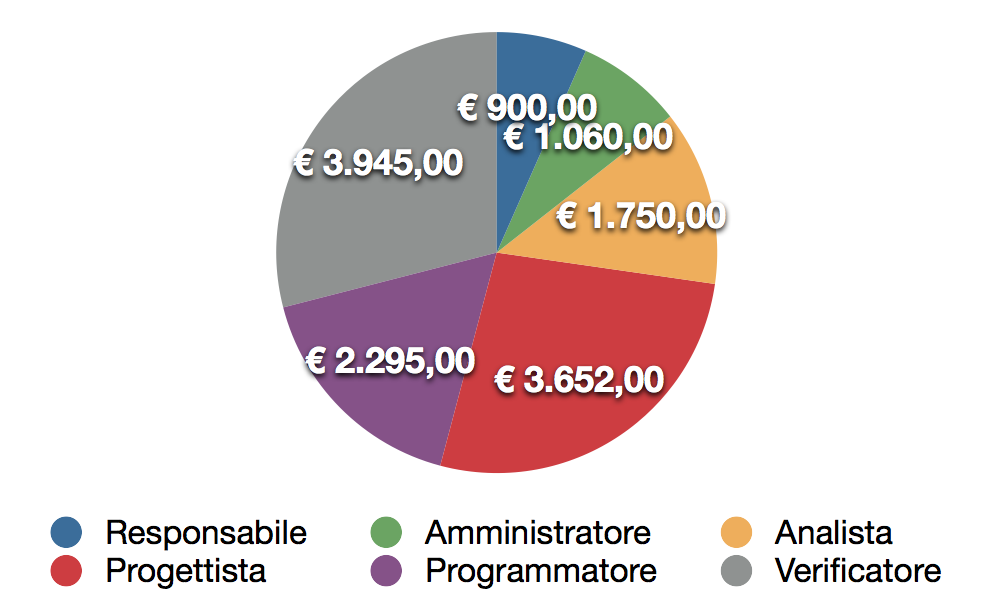
\includegraphics[scale=0.25]{images/costiPerRuoloConsuntivo.png} % vedi Lateximpazienye pg67
\caption{Costi totali per ruolo}
\label{costiTotPerRuoloCons}
\end{figure}


\newpage

\subsection{Analisi dei costi del business model}

Di seguito si riportano costi e guadagni previsti dal business model.

\subsubsection{Costi iniziali}
\begin{itemize}
	\item \textbf{Primo sviluppo del software:} 13602 \EUR.
	\item \textbf{Nuove funzionalità tecniche:} (se ci sono)
	\item \textbf{Consulenza legale:} (se ci servirà)
	\item \textbf{Campagna di marketing:} (...)
\end{itemize}


\subsubsection{Costi fissi}

\begin{itemize}
	\item \textbf{Manutenzione acquisto o la locazione del server:} (...)
\end{itemize}

\subsubsection{Costi variabili}

\red{//TODO?}

\subsubsection{Utenti e guadagni previsti}

\red{//TODO}

\subsubsection{Analisi di Breakeven}

\red{NON SO SE LA FARÒ}

\section{Consuntivo finale del progetto}

Di seguito è riportato il riassunto del quantitativo orario che ogni risorsa ha dedicato al progetto, l'indicazione del costo medio orario (CMO) ed un prospetto indicante i costi totali sostenuti per il progetto.
Questi dati sono stati calcolati nella fase finale del progetto e rappresentano il costo finale del lavoro svolto dalle varie figure professionali impegnate nel progetto per il committente.\\
Il consuntivo deve essere confrontato con il preventivo realizzato nelle fasi preliminari per avere un migliore riscontro delle variazioni rispetto alla previsione iniziale.\\
Viene ora riproposto il CMO delle varie figure professionali impegnate nel progetto:	

\begin{longtable}{ | p{6cm} | p{4.4cm} |}
\caption{Compenso orario delle figure professionali}\\
\hline
\endfirsthead
\multicolumn{2}{r}{\textit{(Continua alla pagina successiva)}}
\endfoot
\multicolumn{2}{l}{\textit{(Continua dalla pagina precedente)}}
\endhead
\hline
\endlastfoot
\textbf{Figura professionale} \ & \textbf{CMO}\\
\hline
\rule[-2mm]{0mm}{0.7cm}
Capo progetto & \EUR \ 40 \\
\hline
\rule[-2mm]{0mm}{0.7cm}
Esperto sicurezza & \EUR \ 28 \\
\hline
\rule[-2mm]{0mm}{0.7cm}
Esperto infrastrutture informatiche & \EUR \ 25 \\
\hline
\rule[-2mm]{0mm}{0.7cm}
Capo programmatore & \EUR \ 30 \\
\hline
\rule[-2mm]{0mm}{0.7cm}
Esperto gamification & \EUR \ 25 \\
\hline
\end{longtable}

Dopo aver osservato il compenso orario per ogni figura impegnata nel progetto viene visualizzato il costo totale dato dal lavoro di ognuna di esse. Tra parentesi possiamo notare le variazioni effettuate dal preventivo stimato nella sezione \virgolette{Pianificazione}. \red{mettere un ref plz}

\begin{longtable}{ | p{6cm} | p{3.5cm} | p{4cm} |}
\caption{Consuntivo costi per ogni figura professionale}\\
\hline
\endfirsthead
\multicolumn{3}{r}{\textit{(Continua alla pagina successiva)}}
\endfoot
\multicolumn{3}{l}{\textit{(Continua dalla pagina precedente)}}
\endhead
\hline
\endlastfoot
\textbf{Figura professionale} \ & \textbf{Ore consuntivate} \ & \textbf{Costi consuntivati} \\
\hline
\rule[-2mm]{0mm}{0.7cm}
Capo progetto & 90 (\textbf{-6}) & \EUR \ 3.600 (\textbf{-240})\\
\hline
\rule[-2mm]{0mm}{0.7cm}
Esperto sicurezza & 126 (\textbf{-4}) & \EUR \ 3.528 (\textbf{-112})\\
\hline
\rule[-2mm]{0mm}{0.7cm}
Esperto infrastrutture informatiche & 77 (\textbf{+2}) & \EUR \ 1.925 (\textbf{+50})\\
\hline
\rule[-2mm]{0mm}{0.7cm}
Capo programmatore & 90 & \EUR \ 2.700 \\
\hline
\rule[-2mm]{0mm}{0.7cm}
Esperto gamification & 108 (\textbf{+4}) &  \EUR \ 2.700 (\textbf{+100}) \\
\hline
\rule[-2mm]{0mm}{0.7cm}
\textbf{Totale} & \textbf{491} (\textbf{-4}) & \textbf{\EUR \ 14.453} (\textbf{-202}) \\
\hline
\end{longtable}

Si analizzano ora le variazioni alle ore e ai costi preventivati. In generale le ore impiegate hanno rispecchiato la pianificazione iniziale abbastanza fedelmente. Le variazioni sono state minime per ogni ruolo in particolare:

\begin{itemize}
	\item Il \textbf{capo progetto} e l'\textbf{esperto di sicurezza} hanno sostenuto un numero di ore leggermente inferiore a quelle previste in fase di pianificazione. Questo dovuto probabilmente ad una sovrastima iniziale per quanto riguarda il controllo del progetto e l'analisi della situazione della sicurezza nel lavoro.
	\item L'\textbf{esperto in infrastrutture informatiche} e l'\textbf{esperto gamification:} hanno svolto un numero di ore leggermente maggiore rispetto al preventivo. Le ore in eccesso sono state svolte per contrastare una leggera sottostima nella pianificazione, soprattutto per quanto riguarda l'analisi dei concorrenti nell'ambito della sicurezza e gamification svolta.
\end{itemize}

Date queste variazioni sono state svolte 4 ore in meno rispetto a quelle totali preventivate, fatto che ha portato ad una appena percettibile diminuzione dei costi totali.\\

Si riassumono infine le variazioni nei costi dal punto di vista delle varie fasi svolte nello sviluppo del progetto nella tabella seguente.


\begin{longtable}{ | p{6cm} | p{4.4cm} |}
\caption{Consuntivo costi per fase di progetto}\\
\hline
\endfirsthead
\multicolumn{2}{r}{\textit{(Continua alla pagina successiva)}}
\endfoot
\multicolumn{2}{l}{\textit{(Continua dalla pagina precedente)}}
\endhead
\hline
\endlastfoot
\textbf{Fase di progetto} \ & \textbf{Costi consuntivati}\\
\hline
\rule[-2mm]{0mm}{0.7cm}
Analisi e pianificazione iniziale & \EUR \ 1.000 \\
\hline
\rule[-2mm]{0mm}{0.7cm}
Analisi di mercato & \EUR \ 2.954 (\textbf{-86})\\
\hline
\rule[-2mm]{0mm}{0.7cm}
Studio di fattibilità & \EUR \ 2.640 (\textbf{+60}) \\
\hline
\rule[-2mm]{0mm}{0.7cm}
Progettazione business model & \EUR \ 5.649 (\textbf{-136})\\
\hline
\rule[-2mm]{0mm}{0.7cm}
Stima rischi/Stima costi & \EUR \ 2.210 (\textbf{-40}) \\
\hline
\rule[-2mm]{0mm}{0.7cm}
\textbf{Totale} & \textbf{\EUR \ 14.453} (\textbf{-202}) \\
\hline
\end{longtable}

Come si può notare le variazioni prima descritte hanno avuto ripercussioni minime nei costi del progetto nelle varie fasi. Vi è stato un leggero aumento dei costi nella fase in cui si è andato ad analizzare il mondo della sicurezza nel lavoro, che dato l'argomento è risultato molto vasto.\\
Le diminuzioni dei costi negli altri ambiti del progetto sono da imputare principalmente alla sovrastima iniziale nelle ore previste per il capo progetto, che essendo la figura professionale con CMO più elevato comporta conseguenze maggiori nei costi rispetto agli altri ruoli.

\end{document}
